\documentclass{scrartcl}

%% support for CMYK color model. However, colors become bland when enabled
\usepackage[cmyk]{xcolor}
%\usepackage[cmyk]{pgf-cmykshadings}

%%
%% Libraries and packages used by the tikz files
%%

\usepackage{fdsymbol}

\usepackage{tikz}
\usepackage{ifthen}
\usepackage{circuitikz}

% listings package used for verbatim environments
\usepackage{listings}
\lstset{basicstyle=\ttfamily}

\usetikzlibrary{shapes,
                arrows,
                shadows.blur,
                fit,
                chains,
                fadings,
                patterns,
                decorations.pathmorphing,
                decorations.markings,
                shapes,
                scopes,
                backgrounds}

%%
%% TikZ fading definitions
%%

%%
% Fading used in timeline diagrams
%
\begin{tikzfadingfrompicture}[name=timeline fade right]
	\shade[left color=transparent!0,
	       right color=transparent!60] (0,0) rectangle (2,2);
\end{tikzfadingfrompicture}

%%
% Fading used in flow charts
%
\begin{tikzfadingfrompicture}[name=flow fade]
	\shade[left color=transparent!0,
	       right color=transparent!60] (0,0) rectangle (2,2);
\end{tikzfadingfrompicture}

\newcounter{decrhelper}


\begin{tikzfadingfrompicture}[name=flow fade]
	\shade[left color=white,
	       right color=transparent!15] (0,0) rectangle (2,2);
\end{tikzfadingfrompicture}

% A4: 21.0 × 29.7
\usepackage[paperwidth=212mm, paperheight=299mm]{geometry}

% clickable URLs
\usepackage[pdftex,hidelinks=true]{hyperref}
\urlstyle{same}

\begin{document}

../../img/tikz-common.tex

\begin{titlepage}
\thispagestyle{empty}

\begin{tikzpicture}[remember picture,overlay]

	\draw [fill=white]
		(current page.south west) rectangle (current page.north east);

	\tikzstyle{section} = [minimum width=212mm, outer sep=0]
	\tikzstyle{user}    = [minimum width=5.25cm, minimum height=4cm, outer sep=0]

	\definecolor{techcolor}      {rgb}{0.721,0.767,0.855}
	\definecolor{sculptcolor}    {rgb}{0.691,0.658,0.691}
	\definecolor{ecosystemcolor} {rgb}{0.74,0.825,0.691}
	\definecolor{usercolor}      {rgb}{0.784,0.614,0.601}
	\definecolor{linkcolor}      {rgb}{0.0,0.1,0.6}

	%
	% Genode as technology
	%
	\path (current page.north)
		node[below=0cm, anchor=north, section, minimum height=7cm] (techoutline) {};

	\path (techoutline.west) -- coordinate[pos=0.5]  (mid)    (techoutline.east);
	\path (techoutline.west) -- coordinate[pos=0.4] (lefty)  (techoutline.east);
	\path (techoutline.west) -- coordinate[pos=0.6] (righty) (techoutline.east);

	\path (techoutline.south)+(0,5ex)  coordinate (southup);
	\path (techoutline.south)+(0,-0ex) coordinate (southdown);

	\tikzstyle{land} = [fill, left color=white, right color=white, inner color=white, path fading=flow fade, rounded corners=0]
	\path[land, opacity=1, inner color=techcolor!50!white, outer color=techcolor]
		(techoutline.north west) --
		(techoutline.north east) --
		(techoutline.south east)
		.. controls +(-6ex,0ex) and +(6ex, 0ex) .. (righty |- southdown)
		.. controls +(-6ex,0ex) and +(6ex, 0ex) .. (mid    |- southup)
		.. controls +(-6ex,0ex) and +(6ex, 0ex) .. (lefty  |- southdown)
		.. controls +(-6ex,0ex) and +(6ex, 0ex) ..
		(techoutline.south west) --cycle;

	%
	% Sculpt OS as showcase
	%
	\path (techoutline.south)
		node[below=0cm, anchor=north, section, minimum height=14.5cm] (sculptoutline) {};

	\path (sculptoutline.north)+(0,5ex)  coordinate (northup);
	\path (sculptoutline.north)+(0,-0ex) coordinate (northdown);
	\path (sculptoutline.south)+(0,5ex)  coordinate (southup);
	\path (sculptoutline.south)+(0,-0ex) coordinate (southdown);

	\path[land, opacity=1, inner color=sculptcolor!70!white, outer color=sculptcolor]
		(sculptoutline.north west)
		.. controls +(6ex,0ex) and +(-6ex, 0ex) .. (lefty  |- northdown)
		.. controls +(6ex,0ex) and +(-6ex, 0ex) .. (mid    |- northup)
		.. controls +(6ex,0ex) and +(-6ex, 0ex) .. (righty |- northdown)
		.. controls +(6ex,0ex) and +(-6ex, 0ex) ..
		(sculptoutline.north east) --
		(sculptoutline.south east)
		.. controls +(-6ex,0ex) and +(6ex, 0ex) .. (righty |- southdown)
		.. controls +(-6ex,0ex) and +(6ex, 0ex) .. (mid    |- southup)
		.. controls +(-6ex,0ex) and +(6ex, 0ex) .. (lefty  |- southdown)
		.. controls +(-6ex,0ex) and +(6ex, 0ex) ..
		(sculptoutline.south west) --cycle;

	%
	% Ecosystem
	%
	\path (sculptoutline.south)
		node[below=0cm, anchor=north, section, minimum height=8.4cm] (ecooutline) {};

	\path (ecooutline.north)+(0,5ex)  coordinate (northup);
	\path (ecooutline.north)+(0,-0ex) coordinate (northdown);
	\path (ecooutline.south)+(0,5ex)  coordinate (southup);
	\path (ecooutline.south)+(0,-0ex) coordinate (southdown);

	\path[land, opacity=1, inner color=ecosystemcolor!50!white, outer color=ecosystemcolor]
		(ecooutline.north west)
		.. controls +(6ex,0ex) and +(-6ex, 0ex) .. (lefty  |- northdown)
		.. controls +(6ex,0ex) and +(-6ex, 0ex) .. (mid    |- northup)
		.. controls +(6ex,0ex) and +(-6ex, 0ex) .. (righty |- northdown)
		.. controls +(6ex,0ex) and +(-6ex, 0ex) ..
		(ecooutline.north east) --
		(ecooutline.south east) --
		(ecooutline.south west) -- cycle;

	\path (techoutline.north west)
		node[inner sep=2ex, anchor=north west, font=\normalsize \sffamily, color=white,
			 opacity=1, scale=2] (genodetitle) {GENODE Operating System Framework};

	\path (techoutline.north east)
		node[inner sep=2ex, anchor=north east, font=\normalsize \sffamily, color=black,
		     opacity=0.5, scale=2] {Technology};

	\path (sculptoutline.north west)
		node[inner sep=2ex, anchor=north west, font=\normalsize \sffamily, color=white,
			 opacity=1, scale=2] (sculpttitle) {Sculpt OS};

	\path (sculptoutline.north east)
		node[inner sep=2ex, anchor=north east, font=\normalsize \sffamily, color=black,
			 opacity=0.5, scale=2] (showcasetitle) {Showcase};

	\path (sculpttitle) -- coordinate (slogan) (showcasetitle);
	\path (slogan) node[font=\normalsize \sffamily, color=white, scale=1.1]
		{ Sculpting Your custom-tailored OS from first principles };

	\path (ecooutline.north east)
		node[inner sep=2ex, anchor=north east, font=\normalsize \sffamily, color=black,
		     opacity=0.5, scale=2] {Ecosystem};

	\tikzstyle{bullet} = [inner ysep=0.7ex, anchor=north west, font=\normalsize \sffamily,
	                      color=black, opacity=1, scale=1.2]

	\path (genodetitle.south west)+(4ex,-2ex) coordinate (banchor);
	\path (banchor.south west) node[bullet] (banchor) { Clean-slate microkernel architecture, not Unix-based };
	\path (banchor.south west) node[bullet] (banchor) { System organized as (dynamic) hierarchy of sandboxes };
	\path (banchor.south west) node[bullet] (banchor) { Resource checks and balances, default-deny, capability-based };
	\path (banchor.south west) node[bullet] (banchor) { Systematic quantifyable risk by clear-cut component relationships };
	\path (banchor.south west) node[bullet] (banchor) { ARM, x86, RISC-V };

	%
	% App-specific TCB
	%
	\path (techoutline.east) node[anchor=east, scale=0.75, outer sep=1cm, yshift=-4ex] (tcb)
		{\includegraphics[width=5.3cm]{app_specific_tcb.pdf}};

	%
	% Screenshots
	%
	\tikzstyle{screenshot} = [blur shadow={shadow blur steps=5,shadow xshift=.0ex,
	                          shadow yshift=-0.5ex,
	                          shadow blur radius=0.25ex},
	                          inner sep=0.5ex]

	\path (current page.center |- sculptoutline.north)+(-4ex,-17ex) node[anchor=north east, screenshot] (sculptpc)
		{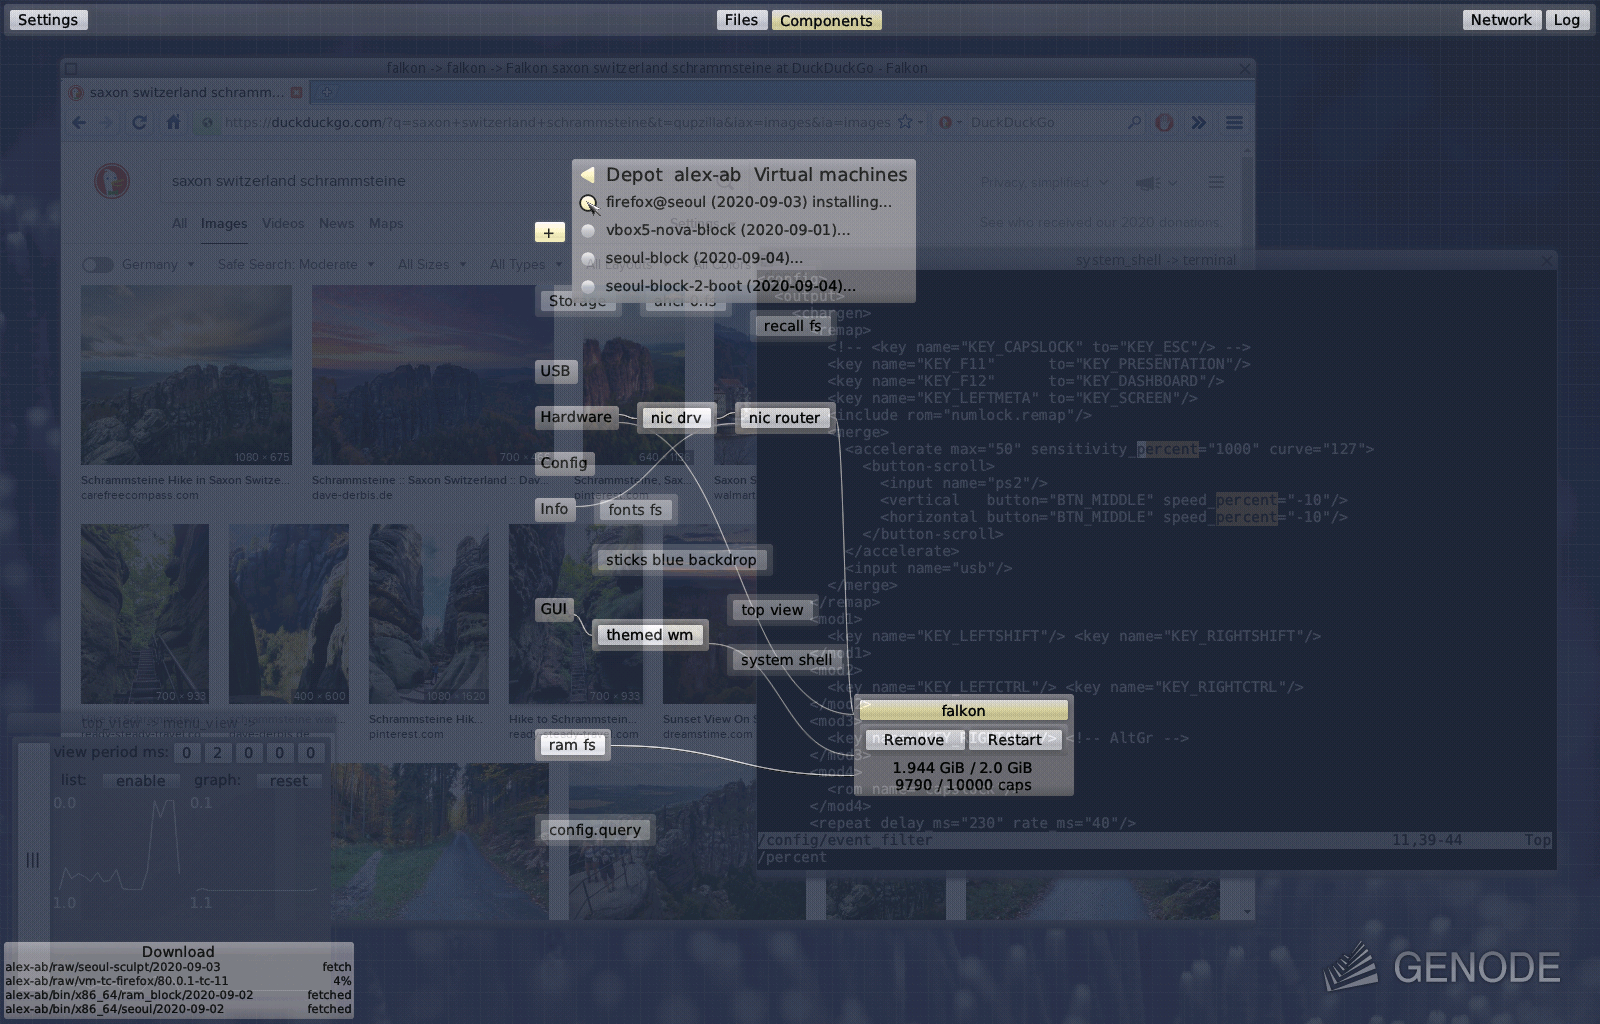
\includegraphics[width=8.0cm]{sculpt_2020-09-16.png}};

	\path (current page.center |- sculptoutline.north)+(4ex,-17ex) node[anchor=north west, screenshot] (phonesection)
		{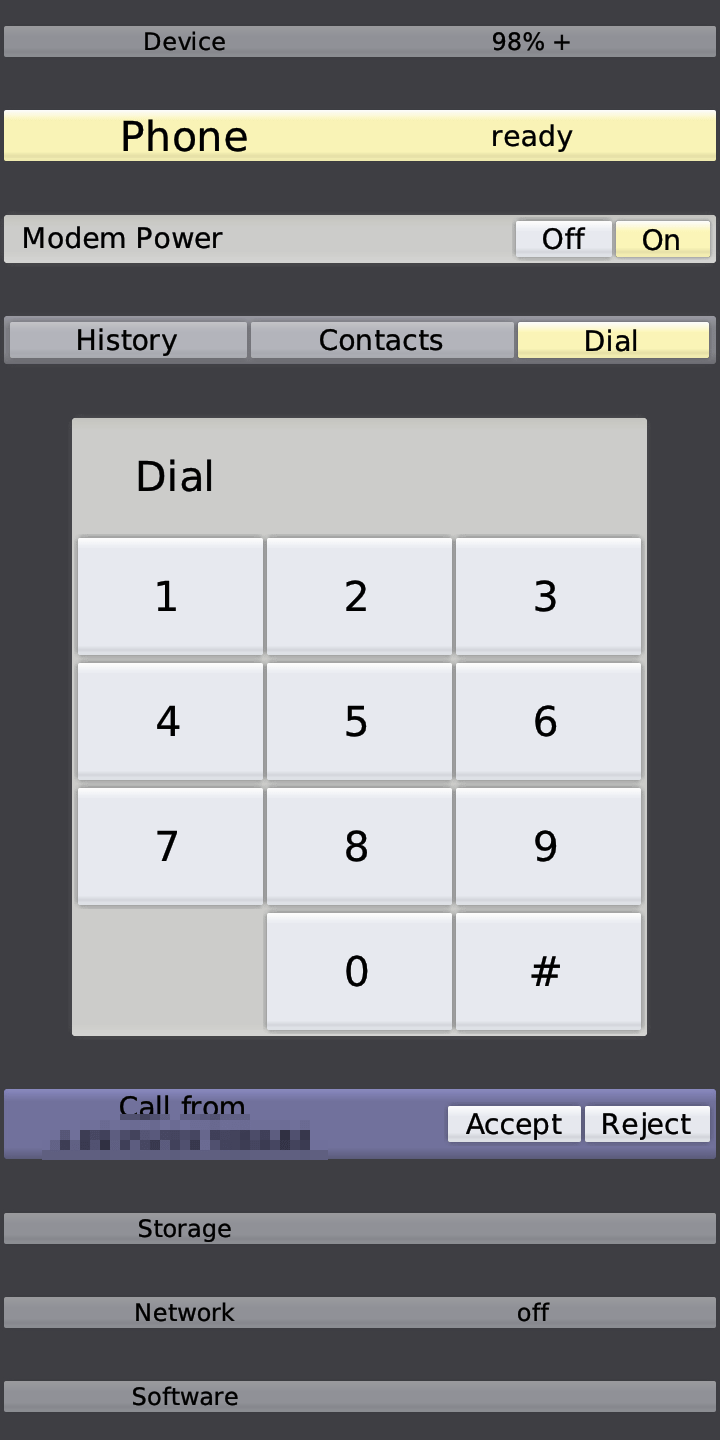
\includegraphics[width=2.5cm]{pinephone_phone_section.png}};

	\path (phonesection.east) node[right=1ex, screenshot] (softwaresection)
		{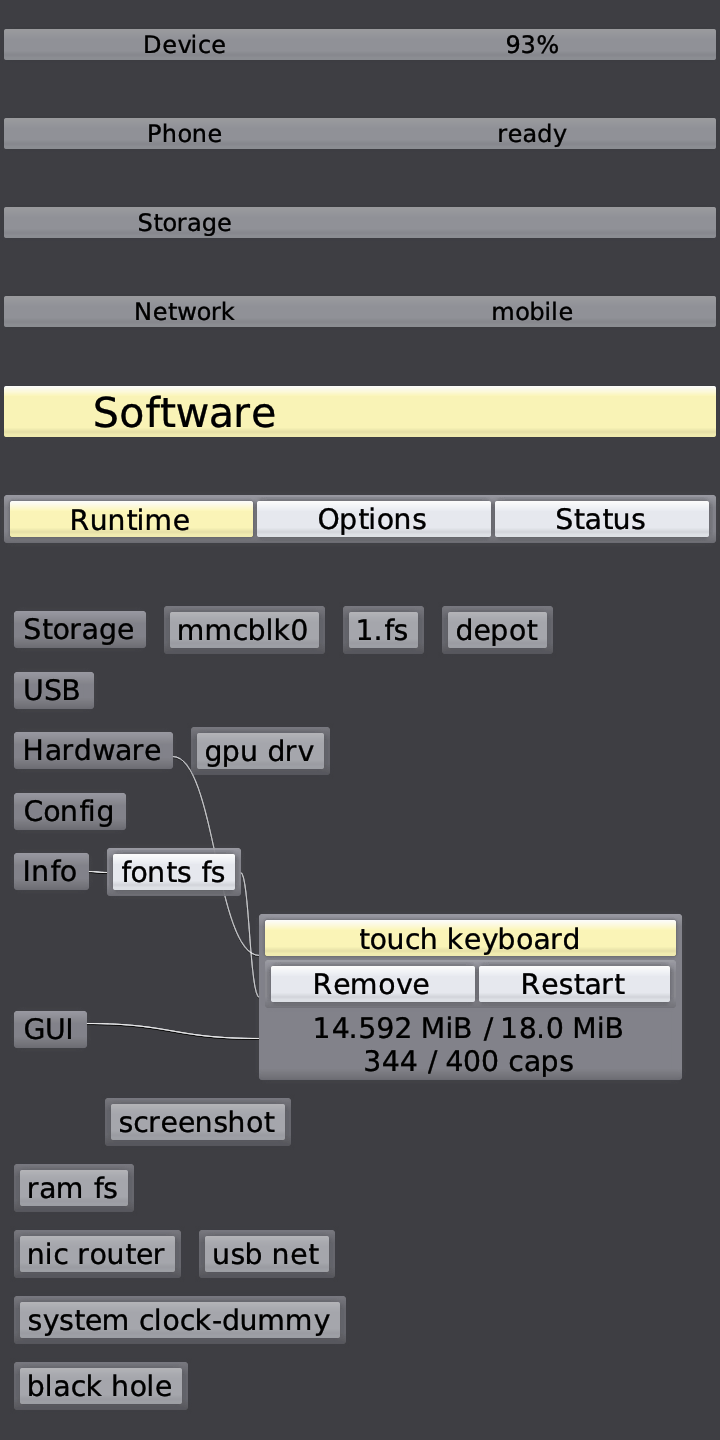
\includegraphics[width=2.5cm]{pinephone_software_section.png}};

	\path (softwaresection.east) node[right=1ex, screenshot] (morph)
		{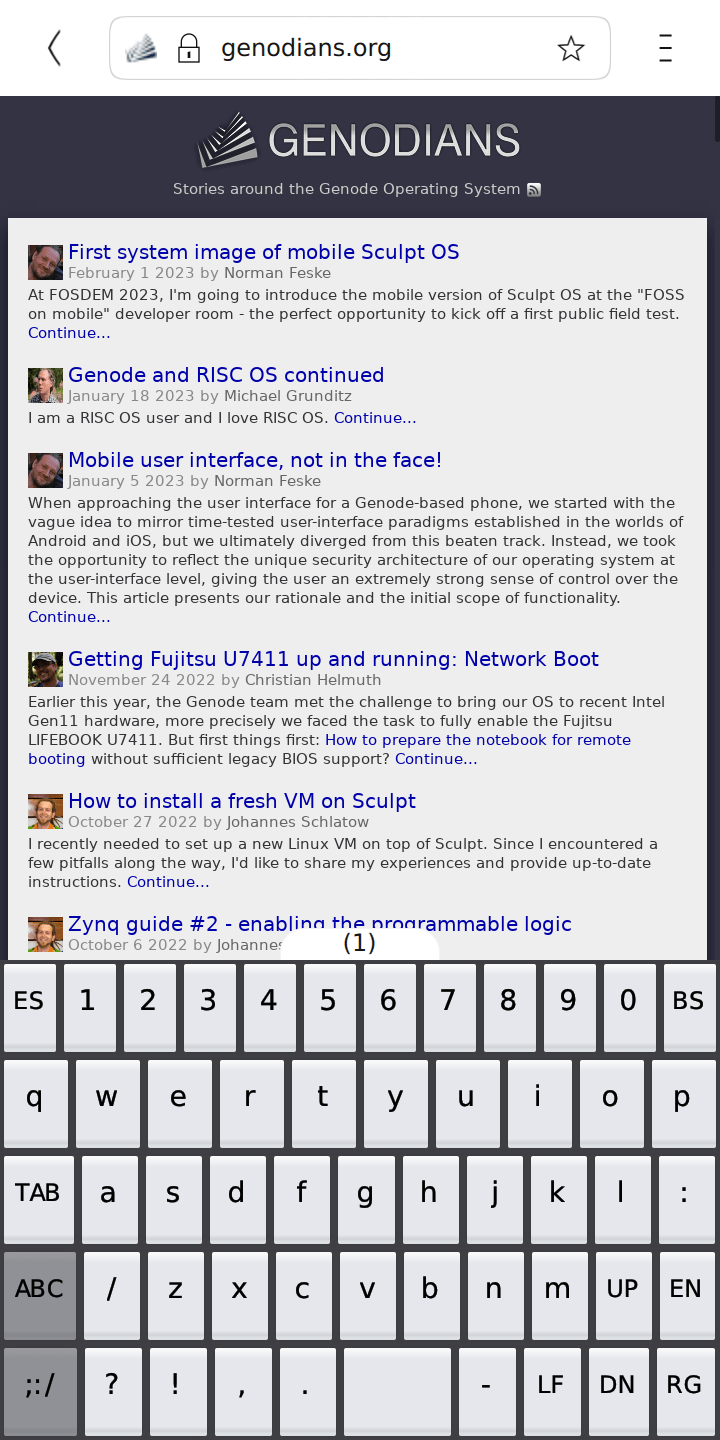
\includegraphics[width=2.5cm]{pinephone_morph.png}};

	\path (sculptpc.north) node[anchor=south, font=\normalsize \sffamily,
	                            color=black, opacity=1, scale=1.2] {Intel PC};

	\path (sculptpc.south) node[inner sep=1ex, anchor=north, font=\normalsize \sffamily,
	                              color=black, opacity=1, scale=1] {VirtualBox available as component};

	\path (softwaresection.south) node[inner sep=1ex, anchor=north, font=\normalsize \sffamily,
	                              color=black, opacity=1, scale=1] {Cold boot takes only 5 seconds};

	\path (softwaresection.north) node[anchor=south, font=\normalsize \sffamily,
	                              color=black, opacity=1, scale=1.2] {PinePhone};

	\path (sculpttitle.south west |- sculptpc.south)+(4ex,-9ex) coordinate (banchor);

	\path (banchor.south west) node[bullet] (banchor) { Attack surface reduced by 99\% };
	\path (banchor.south west) node[bullet] (banchor) {
		Autonomy from dominating software-platform vendors by escaping the security-update treadmill };
	\path (banchor.south west) node[bullet] (banchor) { Integrity-protected on-target package management, system update, and rollback };
	\path (banchor.south west) node[bullet] (banchor) { Security functions: file-encryption vault, WireGuard VPN };
	\path (banchor.south west) node[bullet] (banchor) { Linux drivers as sandboxed components };

	\tikzstyle{wwwlink} = [inner ysep=0.7ex, anchor=east, inner xsep=4ex, font=\normalsize \sffamily,
	                      color=linkcolor, opacity=1, scale=1.2]

	\path (ecooutline.north west)+(4ex,-8ex) coordinate (banchor);
	\path (banchor.south west) node[bullet] (banchor) { Interoperable with POSIX, C++, Qt, GNU, Chromium engine, OpenGL, Java ... };
	\path (banchor.south west) node[bullet] (banchor) { Existing OSes usable as virtual machines };
	\path (banchor.south west) node[bullet] (banchor) { Quarterly releases };
	\path (ecooutline.east |- banchor) node[wwwlink] { \url{https://genode.org} };
	\path (banchor.south west) node[bullet] (banchor) { Driven by small team in Germany since 2008 };
	\path (ecooutline.east |- banchor) node[wwwlink] { \url{https://genode-labs.com} };
	\path (banchor.south west) node[bullet] (banchor) { Open Source and commercial licensing };
	\path (ecooutline.east |- banchor) node[wwwlink] { \url{https://github.com/genodelabs} };
	\path (banchor.south west) node[bullet] (banchor) { International community };
	\path (ecooutline.east |- banchor) node[wwwlink] { \url{https://genodians.org} };

	\tikzstyle{userrole} = [inner ysep=3ex, anchor=north, inner xsep=4ex, font=\normalsize \sffamily,
	                      color=white, opacity=1, scale=1.5]

\end{tikzpicture}

\end{titlepage}

\end{document}
